% Requires the package calligra
\newfontfamily{\ovidius}{ovidius demi}
\cxset{style06/.style={%
 name=Chapter,
 numbering=arabic,
 number font-size=LARGE,
 number font-family=ovidius,
 number font-weight=mdweight,
 number color= black!60,
 number before=\kern3.5pt,
 number dot=,
 number after=\hfill\hfill\par\offinterlineskip,
 number position=rightname,
 chapter font-family= ovidius,
 chapter font-weight=normal,
 chapter font-size= LARGE,
 chapter before=\vspace*{2pt}\par\hfill,
 chapter after=,
 chapter color={black!60},
 chapter spaceout=none,
 title margin top=30pt,
 title before=\hfill\par,
 title after=\hfill,
 title font-family=rmfamily,
 title font-color= black!90,
 title font-weight=normalfont,
 title font-size=LARGE,
 title spaceout=none,
 chapter title width=0.6\textwidth,
 chapter title align=centering,
 }}

\cxset{style06}


\chapter{THE RITUALS OF THE MONTHS OF THE YEAR}
\renewcommand{\DefaultLhang}{0.1}
\renewcommand{\LettrineFontHook}{\calligra}
\setlength{\DefaultFindent}{9.5pt}
\setlength{\DefaultNindent}{0pt}
\renewcommand{\LettrineFontHook}{\ovidius}
\lettrine[loversize=0.6]{\textcolor{thegray!60}{C}}{}rist\'obal de Molina’s manuscript titled \emph{Account of the Fables and Rites of the Incas (Relación
de las fábulas y ritos de los incas)}, written aroun 1575 records the rituals that were conducted in Cuzco during the last years of the Inca Empire. An excellent translation was published by
\begin{figure}[ht]
\centering
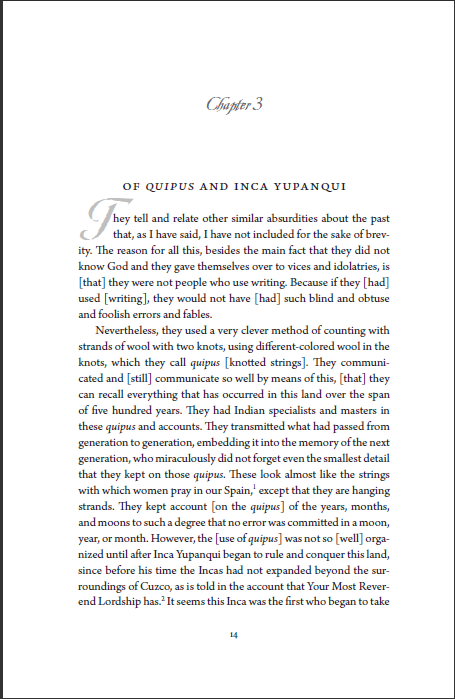
\includegraphics[width=0.45\textwidth]{./chapters/chapter06.png}
\caption{Style 5 sample}
\end{figure}
the University of Texas Press. The translation is by Brian S. Bauer, Vania Smith-Oka and Gabriel E. Cantarutti who did an excellent job. The typesetting attracted my attention by its effective simplicity and I read the book in one evening. The book size is 5.50 x 8.50 in, pages 187. Times Roman, ArnoPro and Ovidius. The Ovidius font was designed by  Thaddeus Szumilas and 
belongs to a family known as eroded fonts. It has found many devoted users especially for book covers.

This template has a lot of potential and I will come back to it and add more key hooks for lettrine settings per letter and font management. They can also come alive with a gold color.

The dropcap in the original book as well as the chapter font is given a worn style (Ovidius Demi font\footnote{Available at the fontpalace website \protect\url{http://www.fontpalace.com/font-download/Ovidius Demi/}}), I guess in order to give it a touch of style reminiscent of a manuscript. It can also look
good using |calligra| and also a bit of color. You can experiment also with many other calligraphic fonts. The example below demonstrates the use of the |calligra| font.
\bigskip

\renewcommand{\LettrineFontHook}{\calligra}
\cxset{chapter opening=anywhere}
\cxset{chapter font-family=calligra}
\cxset{number font-family=calligra}
\cxset{number font-weight=calligra}
\cxset{number font-size=Huge}
\cxset{number before=\kern2.5pt}
\cxset{chapter color=black!90,
          number color=black!90}
\bigskip

\topline

\chapter{OF QUIPUS AND INCA YUPANQUI}

\lettrine[loversize=.6]{\textcolor{orange}{T}}{}he book by Crist\'obal de Molina’s manuscript titled \emph{Account of the Fables and Rites of the Incas (Relación
de las fábulas y ritos de los incas)}, written aroun 1575 records the rituals that were conducted in Cuzco during the last years of the Inca Empire. An excellent translation was published by
\medskip

The dropcap looks as good if not better with the |calligra| font and I have given it a colour to stand out. The chapter number has to be increased in height, so I have used |huge|. The new
settings are shown below:

\begin{verbatim}
\renewcommand{\LettrineFontHook}{\calligra}
\cxset{chapter opening=anywhere}
\cxset{chapter font-family=calligra}
\cxset{number font-family=calligra}
\cxset{number font-weight=calligra}
\cxset{number font-size=Huge}
\cxset{number before=\kern2.5pt}
\cxset{chapter color=black!90,
          number color=black!90}
\end{verbatim}

\cxset{section align=center,
          section numbering=none,
          section font-weight=normalfont,
          section font-family=rmfamily,
          section font-size=large,
          section color=black,
          section font-shape=scshape}


\section{THE SECTIONS}

The sections are typeset in normal font and are centered.

\bottomline 